% \begin{frame}{Logic}
% 	\begin{center}
% 		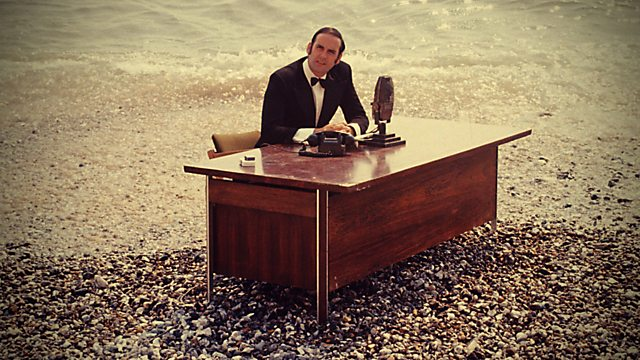
\includegraphics[width=\textwidth]{figures/something_different.jpg}
% 	\end{center}
% 	%We would like to define \textbf{sheaves on arbitrary categories}: in fact, there are presheaves on any category, why shouldn't we have sheaves?
% \end{frame}

\begin{framecard}
	{\color{white}
	\bfseries

	\hugetext{Logic}}
\end{framecard}

\begin{frame}{Logic}
	\textbf{Idea}:
	\begin{center}
		\color{red}
		\bfseries
			sheaves are 'locally defined sets' on a 'site'.
	\end{center}

	\vspace{5ex}

	We are going to see
	\begin{enumerate}
		\item Sites \& topoi
		\item The internal language of a topos of sheaves
		\item The `locally' modality
		\item Logical-flavoured applications: forcing, internalization
	\end{enumerate}
\end{frame}

\begin{frame}{Sites}
	Let $\cat C$ be a small category.
	\begin{definition}
		A \defining{sieve} on $U \tin \cat C$ is a collection $S$ of morphisms $\{U_i \to U\}_{i \in I}$ closed by precomposition on the left:
		\begin{equation*}
			\underbrace{V \to \underbrace{U_i \to U}_{\in S}}_{\implies \in S}
		\end{equation*}
		\setnote{You generate a sieve by choosing some morphisms into $U$ and then closing.}
	\end{definition}

	\begin{definition}<2->
		A \defining{site} is a small category $\cat C$ together with a \defining{Grothendieck topology} $J$, i.e. a choice of sieves for each object $U \tin \cat C$:
		\begin{equation*}
			J(U) = \text{\bfseries covering sieves for $U$}
		\end{equation*}
		\setnote{such that $J(U)$ satisfies some very reasonable conditions.}
	\end{definition}
\end{frame}

\begin{frame}{Sites}
	\begin{definition}
		Let $(\cat C, J)$ be a site.
		A presheaf $F : \cat C^\op \to \Set$ is a sheaf iff for every $U \tin \cat C$ and any \emph{covering sieve} $S \in J(U)$,
		\begin{equation*}
			F(U) \iso \lim F(S).
		\end{equation*}
		\textbf{Warning}: it's not always true that $U \iso \colim S$!
	\end{definition}

	\begin{example}<2->
		For $X$ topological space:
		\begin{eqalign*}
			\Sh X  &= \Sh (\O(X),\, \text{open coverings})\\
			\Psh X &= \Sh (\O(X),\, \text{trivial coverings})
		\end{eqalign*}
	\end{example}
	\onslide<3->{
		\textbf{Takeaway}: locality is not a fixed concept! It depends on the topology, but not the one you expect.
	}
\end{frame}

\begin{frame}{The topos of presheaves}
	Let $X$ be a site. $\Sh X$ inherits a lot of structure from $\Set$:
	\begin{enumerate}
		\item {[Finite]} \textbf{completeness} and \textbf{cocompleteness} (pointwise co/limits)
		\item \textbf{Exponentials}:
		\begin{equation*}
			G^F(U) \iso \Nat(\yo U, G^F) \iso \Nat(\yo U \times F, G)
		\end{equation*}
		\item \textbf{Subobject classifier}: $\Omega(U) =$ `principal covering sieves on $U$'.
		\begin{diagram*}
			P \arrow[tail, swap]{d}{\forall \varphi} \arrow{r}{!} \& 1 \arrow{d}{\true} \&[-3ex] \color{colornote}{*} \arrow[colornote, mapsto]{d}\\
			F \arrow{r}{\exists ! \ulcorner \varphi \urcorner} \& \Omega \& \color{colornote}{1_U}
		\end{diagram*}
		\begin{diagram*}
			\phantom{XXX} \color{colornote}{s \in F(U)} \arrow[colornote, mapsto]{r} \& \color{colornote}{\{ V \nto{f} U \suchthat s\vert_f \in P(V) \}}
		\end{diagram*}%
		Intuition: `ways $s$ enters in $P$ at $U$'.\\
		$P(s)$ true at $U$ \underline{iff} $s$ entered through $1_U$ \underline{iff} $s \in P(U)$ already.
	\end{enumerate}
\end{frame}

\begin{frame}{Internal language of topoi}
	A category satisfying these properties is called an \defining{elementary topos}.\\
	A topos $\simeq$ to a topos of sheaves on a site is called \defining{Grothendieck}.

	\vfill

	The definition is tailored to provide a rich \textbf{internal language}:

	\begin{center}
		\begin{tabularx}{\textwidth}{XX}
			$A$ type & $A$ object\\[1.5ex]
			$t(x) \tin A \, [x \tin X]$ & $X \nto{t} A$\\[1.5ex]
			$\varphi(x) \tin \Prop\,[x \tin X]$ & $X \nto{\varphi} \Omega$ \setnote{(hence $\{x \suchthat \varphi\} \mono X$)}\\[1.5ex]
			%$\lambda y^Y . t(x,y) \tin Y \to A\,[x \tin X]$ & $X \nto{\lambda t} A^Y$\\[1.5ex]
			$\forall/\exists y \tin Y\ \varphi(x, y)\,[x \tin X]$ & \begin{tikzcd}[ampersand replacement=\&, cramped]
				\Omega^{X \times Y} \arrow[shift left=5]{r}{\exists y : Y} \arrow[shift right=2, swap]{r}{\forall y : Y} \& \Omega^Y \arrow[swap]{l}{\pi_Y^*}
			\end{tikzcd}
		\end{tabularx}
	\end{center}
	+ type/term constructors coming from exponentials, limits, colimits, ...

	\vfill
	\color{red}{\bfseries Basically the internal language of $\Set$!}
\end{frame}

\begin{frame}{ Kripke--Joyal semantics}
	Let $X$ be a topological space, $U \subseteq X$, $\varphi, \psi$ formulae of $\Sh X$:
	\vspace{-3ex}
	\begin{center}%
		\begin{tabular}{lcp{45ex}}
			$U \forces \varphi \land \psi$ & \underline{iff} & $U \forces \varphi$ and $U \forces \psi$\\
			$U \forces \varphi \lor \psi$ & \underline{iff} & there exists an open covering $\{U_i\}_{i \in I}$ of $U$ \newline such that $U_i \forces \varphi$ or $U_i \forces \psi$ for every $i \in I$\\
			$U \forces \varphi \hey \psi$ & \underline{iff} & for all $V \subseteq U$, $V \forces \varphi$ implies $V \forces \psi$\\
			$U \forces \forall s \tin F\ \varphi(s)$ & \underline{iff} & for any $s \in F(U)$ and $V \subseteq U$, $V \forces \varphi(s)$\\
			$U \forces \exists s \tin F\ \varphi(s)$ & \underline{iff} & there exists an open covering $\{U_i\}_{i \in I}$ of $U$\newline such that for all $i \in I$ there exists $s_i \in F(U_i)$ such that $U_i \forces \varphi(s_i)$.
		\end{tabular}
	\end{center}
	\onslide<2->{
		This interpretation is \textbf{local}: if $\{U_i\}_{i \in I}$ is an open covering of $U$,
		\begin{equation*}
			U \forces \varphi \sse \text{for every $i \in I$, $U_i \forces \varphi$}
		\end{equation*}
	and \textbf{intuitionistically sound}: if $\varphi \entails \psi$ in HIL, then
		\begin{equation*}
			U \forces \varphi \word{implies} U \forces \psi.
		\end{equation*}
	}
\end{frame}

\begin{frame}{Lawvere--Tierney topologies}
	\begin{definition}
		A \defining{Lawvere--Tierney topology} on a topos $\topos E$ is an operator $\square : \Omega \to \Omega$ such that
		\begin{enumerate}
			\item $\topos E \forces \varphi \hey \square \varphi$ \setnote{(global truth entails local truth)}
			\item $\topos E \forces \square \square \varphi \hey \square \varphi$ \setnote{(stability under refinements)}
			\item If $\topos E \forces \varphi \hey \psi$ then $\topos E \forces \square \varphi \hey \square \psi$ \setnote{(internal soundness)}
		\end{enumerate}
	\end{definition}
	Define $\halfsquare : \topos E \to \topos E$:
	\begin{equation*}
		\halfsquare X := \{ \text{$\square$-singletons of $X$} \}_{\big/ \square (=_X)}
	\end{equation*}
	\vspace{-5.5ex}
	\begin{proposition}
		An LT topology extends to a lex monad $\square = \halfsquare \halfsquare$.
	\end{proposition}
	\begin{definition}
		A \defining{sheaf} in $\topos E$ is a modal type for $\square$, meaning $\square X \iso X$.
	\end{definition}
\end{frame}

\begin{frame}{Topologies on topoi}
	\begin{block}{Facts}
		\begin{enumerate}
			\item Any Lawvere--Tierney topology on $\Psh(\cat C)$ gives rise to a Grothendieck topology on $\cat C$:
			\begin{eqalign*}
				J(U) = \{ \text{$S$ sieve on $U$} \suchthat \text{$\square S = S$}\}.
			\end{eqalign*}
			and viceversa
			\item Moreover, any subtopos $\topos E \ninto{i} \Psh (\cat C)$ is the topos of sheaves for the LT topology induced by the monad $i_* \adj i$.
			\item Hence, for Grothendieck topoi:
			\begin{center}
			\bfseries
				Grothendieck topologies $\equiv$ LT topologies $\equiv$ subtopoi
			\end{center}
			and they all agree on which are the sheaves.
		\end{enumerate}
	\end{block}
	Notice: LT topologies/subtopoi work in non-Grothendieck topoi too!
\end{frame}

\begin{frame}{Forcing}
	% \textbf{Remark}: sheafification is a \emph{localization}, i.e. we introduce new isomorphisms, hence we also enlarge the class of monos $P \nmono{\varphi} X$ such that $\varphi \iso \true_X$:
	% \begin{equation*}
	% 	\square \topos E \forces \varphi \sse \topos E \forces \varphi^\square
	% \end{equation*}
	% where $\varphi^\square$ is the `$\square$-translation', i.e. a recursive application of $\square$ to subformulae $\varphi$.

	% In particular: \textbf{existence is local}.

	\textbf{Idea}: existence is local in a sheaf topos, hence we can define global things by glueing together smaller approximations:
	\vfill
	\textbf{Rough recipe}:
	\begin{enumerate}
		\item Construct a poset $P$ of `finite' approximations of the object, ordered by (reverse) extension
		\item Take a `tautological sheaf' on it: $A(p) = p$
		\item $A$ will be the desired object in $\Sh P$.
	\end{enumerate}
	\vfill
\end{frame}

\begin{frame}{Forcing}
	\begin{example}[Cohen topos]
		We want to construct a model $\mathcal M$ of $\mathsf{ZFC}$ where there exists $A$ such that
		\begin{equation*}
			\mathcal M \forces \N \lneq A \lneq P_{\mathcal M} \N
		\end{equation*}
		Take $B = PP\N$. Then we \emph{force} the above inclusions:
		\begin{enumerate}
			\item $P = $ `partially defined monos $B \nmono{p} 2^\N$', $\mathcal M = \Sh(P, \neg\neg)$,
			\item $A(p) = \{(k, n) \suchthat n \in p(k)\}$,
			\item We get $A \mono \Delta B \times \Delta \N$, one can show defines a mono $\Delta B \mono \Omega^{\Delta \N}$.
		\end{enumerate}
		Then we can prove
		\begin{equation*}
			\Set \forces \N \lneq B \word{implies} \Sh(P, \neg\neg) \forces \Delta\N \lneq \Delta B
		\end{equation*}
		so that
		\begin{equation*}
			\Sh(P, \neg\neg) \forces \Delta \N \neq \Delta B \lneq \Omega^{\Delta \N}.
		\end{equation*}
		{\bfseries\color{colornote}Disclaimer: several details under the rug!}
	\end{example}
\end{frame}

\begin{frame}{Internalization}
	\textbf{Idea}: $\Sh X$ is naturally suited to describe mathematics 'over $X$'.

	\begin{example}[{\cite{blechschmidt2018using}}]
		Commutative algebra done in $\Sh X$ is equivalent to algebraic geometry done over $X$.
	\end{example}
	\begin{example}[Bohr topos]
		Let $A$ be a non-commutative $C^*$-algebra.
		Classical physics done in
		\begin{equation*}
			\operatorname{Bohr}(A) = \Sh(\text{commutative subalgebras of $A$})
		\end{equation*}
		is equivalent to quantum physics done over $A$.
	\end{example}
	\begin{example}[{Scott topos \cite{capucci2020internal}}]
		Let $(X,\Sigma, \mathbb P)$ be a probability space. Classical calculus done in
		\begin{equation*}
			\operatorname{Scott}(X) = \Sh (\Sigma / \ker \P)
		\end{equation*}
		is equivalent to stochastic calculus done over $X$. \setnote{WIP!}
	\end{example}
\end{frame}

\begin{frame}{Systems theory}
	\textbf{Idea}: the internal language of $\Psh(\cat S)$ can express constraints on the behaviour of a system (modelled by a site $\cat S$).

	\begin{example}
		Let $B \tin \Psh(\cat S)$, with input/outputs maps $I \nfrom{f} B \nto{g} O$. Consider:
		\begin{equation*}
			\texttt{Tot}(b) :\equiv \forall i \tin I\ \exists o \tin O\ (i = f(b) \land g(b) = o).
		\end{equation*}
		Then `total behaviours in $B$' = $\{ b \tin B \suchthat \texttt{Tot}(b)\} \mono B$.
	\end{example}
	\begin{example}
		Let $B \tin \Psh (\cat S)$, let $\square$ be the `locally' modality better suited for $\cat S$. Then
		\begin{eqalign*}
			\texttt{Extensional} &:\equiv `\text{$S \to \halfsquare S$ is injective}`\\
			\texttt{Non-generative} &:\equiv `\text{$S \to \halfsquare S$ is surjective}`
		\end{eqalign*}
	\end{example}
	Greatly expounded in \cite{schultz2019temporal}.
\end{frame}
